% ---------------------------------------          Preamble
\documentclass[
	fontsize=12pt,
	paper=a4,
	twoside=false,
	numbers=noenddot,
	plainheadsepline,
	toc=listof,
	toc=bibliography
]{scrartcl}

\usepackage[english]{babel} 

\usepackage{amssymb}
\usepackage{amsmath}
\usepackage{array}

\usepackage{placeins}
\usepackage{float}

\usepackage{graphicx}
\restylefloat{figure}
\usepackage{caption}
\usepackage{subcaption}
%\usepackage{subfigure} 
\usepackage{tikz}

%\usepackage{pdfpages} % insert images saved as pdf

% pseudo algorithms
\usepackage[ruled,vlined]{algorithm2e}

% lscape.sty Produce landscape pages in a (mainly) portrait document.
\usepackage{lscape}

\usepackage{hyperref}

\setlength{\parindent}{0pt}

\usepackage[sort, numbers]{natbib}
% ---------------------------------------          New commands
%\newcommand{\argmin}{\operatornamewithlimits{argmin}}
\def\argmax{\mathop{\rm argmax}}						% argmax
\def\argmax{\mathop{\rm argmin}}						% argmin
\def\median{\mathop{\rm median}} 						% median
\def\dist{\mathop{\rm dist}} 						    % dist


\usepackage{array}
\newcolumntype{L}[1]{>{\raggedright\let\newline\\\arraybackslash\hspace{0pt}}m{#1}}
\newcolumntype{C}[1]{>{\centering\let\newline\\\arraybackslash\hspace{0pt}}m{#1}}
\newcolumntype{R}[1]{>{\raggedleft\let\newline\\\arraybackslash\hspace{0pt}}m{#1}}


\usepackage{xcolor} 
\newcommand\ToDo[1]{\textcolor{red}{#1}} 

% ------------------------------------------------------------------------------------------------------------
% ------------------------------------------------------------------------------------------------------------
% ------------------------------------------------------------------------------------------------------------

\begin{document}

\pagestyle{plain}
\pagenumbering{arabic}

% ------------------------------------------------------------------------------------------------------------
% ---------------------------------------          Title
\title{Graph Matching Framework}
\author{Ekaterina Tikhoncheva}
\date{} 

\maketitle 

% ------------------------------------------------------------------------------------------------------------
% ---------------------------------------          Introduction
%This notes are a short description of graph matching model applied for finding feature correspondences between two images.
%
%% Inhaltsverzeichnis erzeugen
%\tableofcontents
%\newpage

% ------------------------------------------------------------------------------------------------------------
% ---------------------------------------        Problem Statement
\section{Problem statement} \label{sec:prob_stat}
Consider two undirected weighted graphs $G^I = (V^I, E^I, D^I)$ and $G^J = (V^J, E^J, D^J)$, where $V$, $E$, $D$ denote set of nodes,
set of edges and set of node attributes respectively. We assume the situation, where $|V^I|=n_1$, $|V^J|=n_2$ and $n_1$ not necessary equal to $n_2$.

The aim of graph matching is to find a subset of possible node correspondences, which maximizes the similarity value between two graphs. Such a subset can be represented by a binary vector $x\in \{0,1\}^{n_1n_2}$, where $x_{(j-1)n_1+i}=1$, if node $v_i\in V^I$ is matched to node $u_j\in V^J$, and $x_{(j-1)n_1+i}=0$ otherwise. For simplicity we will write further $x_{ij}$ instead of $x_{(j-1)n_1+i}$.

To measure a similarity between graphs we define two similarity functions: \emph{nodes similarity function} (first-order similarity) $s_V(v_i, u_j),\ v_i\in V^I, u_j\in V^J$ and \emph{edge similarity function} (second-order similarity) $s_E(e_{ii\prime}, e_{jj\prime}),\ e_{ii\prime}\in E^I, e_{jj\prime}\in E^J$. Both functions can be combined in one \emph{similarity} or \emph{affinity matrix $S\in\mathbb{R}^{n_1n_2\times n_1n_2}$}, whose diagonal elements are $s_V(v_i, u_j)$ and non-diagonal elements are $s_E(e_{ii\prime}, e_{jj\prime})$.


Using this notation one can formulate a \emph{one-to-one Graph Matching Problem} \textbf{GMP} as an quadratic optimization problem \cite{Cho2014_Haystack, Cho2010_RRWM, Cho2012_ProgressiveGM, Conte2004}: 
\begin{alignat}{2}
    &     && \argmax_x{x^TSx}                           \notag\\
    & \text{s.t. } &&  x\in \{0,1\}^{n_1n_2}            \label{QIP:2}\\
    &             &&  \sum_{i=1\dots n_1} x_{ij} = 1    \label{QIP:3}\\
    &             &&  \sum_{j=1\dots n_2} x_{ij} = 1    \label{QIP:4}
 \end{alignat}
 
The maximum number of possible matches is equal to $\min(n_1, n_2)$. That means, in case when $n_1\not = n_2$, only one of the conditions (\ref{QIP:3}) or (\ref{QIP:4}) will be fulfilled.

A Quadratic Optimization Problem is known to be \emph{NP}-hard \cite{Sahni1974}. This limits greatly the size of a graph, for which a exact solution can be calculated in reasonable time. Due to this there are a number of algorithms \cite{Cho2014_Haystack, Cho2010_RRWM, Cho2012_ProgressiveGM, Chui2003, Suh_CVPR2015}, that solve graph matching problem inexact.

Unfortunately, most of the algorithms have the two following problems:
\begin{enumerate}
\item they are still limited in size of permissible graphs. Experiments in most of the papers consider graphs with up to $100$ nodes \cite{Cho2014_Haystack, Cho2010_RRWM, Cho2012_ProgressiveGM}
\item possible presence of outliers can reduce the accuracy of matching algorithm \cite{Suh_CVPR2015}.
\end{enumerate}  

Our main aim was to develop a framework, which would allow an existing graph matching algorithm to cope with both problems.


% ------------------------------------------------------------------------------------------------------------
% ---------------------------------------        Approach
\section{Approach}

The main idea of our approach is to create a flexible multi-scale matching framework, that could improve the speed of
theoretically any matching algorithm for large graphs and additionally increase their accuracy. 

Given initial graphs $G^I$ and $G^J$ we create for each of them coarse representative graphs $A^I$, $A^J$. Each node of such a graph represents a subgraph of the initial graph. We refer further to nodes of the coarse graphs $A^I$, $A^J$ as \emph{anchor nodes} or just \emph{anchors} and to the graphs themself as \emph{anchor graphs}.

Initial graphs with corresponding anchor graphs build a two level structure (see Fig. \ref{fig:2levels}): initial graphs (or \emph{fine graphs}) represent a lower level and anchor graphs represent a higher level.  

In case of large $G^I$ and $G^J$ graphs, where existing inexact solution techniques are difficult to apply due to time and storage complexity, their anchor graphs can be constructed small enough to not have these problems. That makes it possible, to find a solution of GMP on the higher level fast. 

Ones the matching problem is solved on the higher level, we get the correspondences between the subgraphs of the initial graphs, which are also much smaller compared to the complete graphs. Solving after that GMP for pairs of subgraphs lead us to the desirable correspondences between nodes of fine graphs.

Obviously, the accuracy of such two level matching approach depends heavily on the partition of the initial graphs into subgraphs and on the matching quality of the anchor graphs. To make the approach more robust we integrate the result of matching on the lower level into a graph partition algorithm and repeat the whole scheme several times till convergence.

In our work we concentrate ourself on the task of finding feature correspondences between two images. In the next sections we describe in detail the construction of initial graphs from given images and corresponding anchor graphs together with the matching algorithm on both levels and propagation of the matching results between the levels.

\begin{figure}
	\centering
	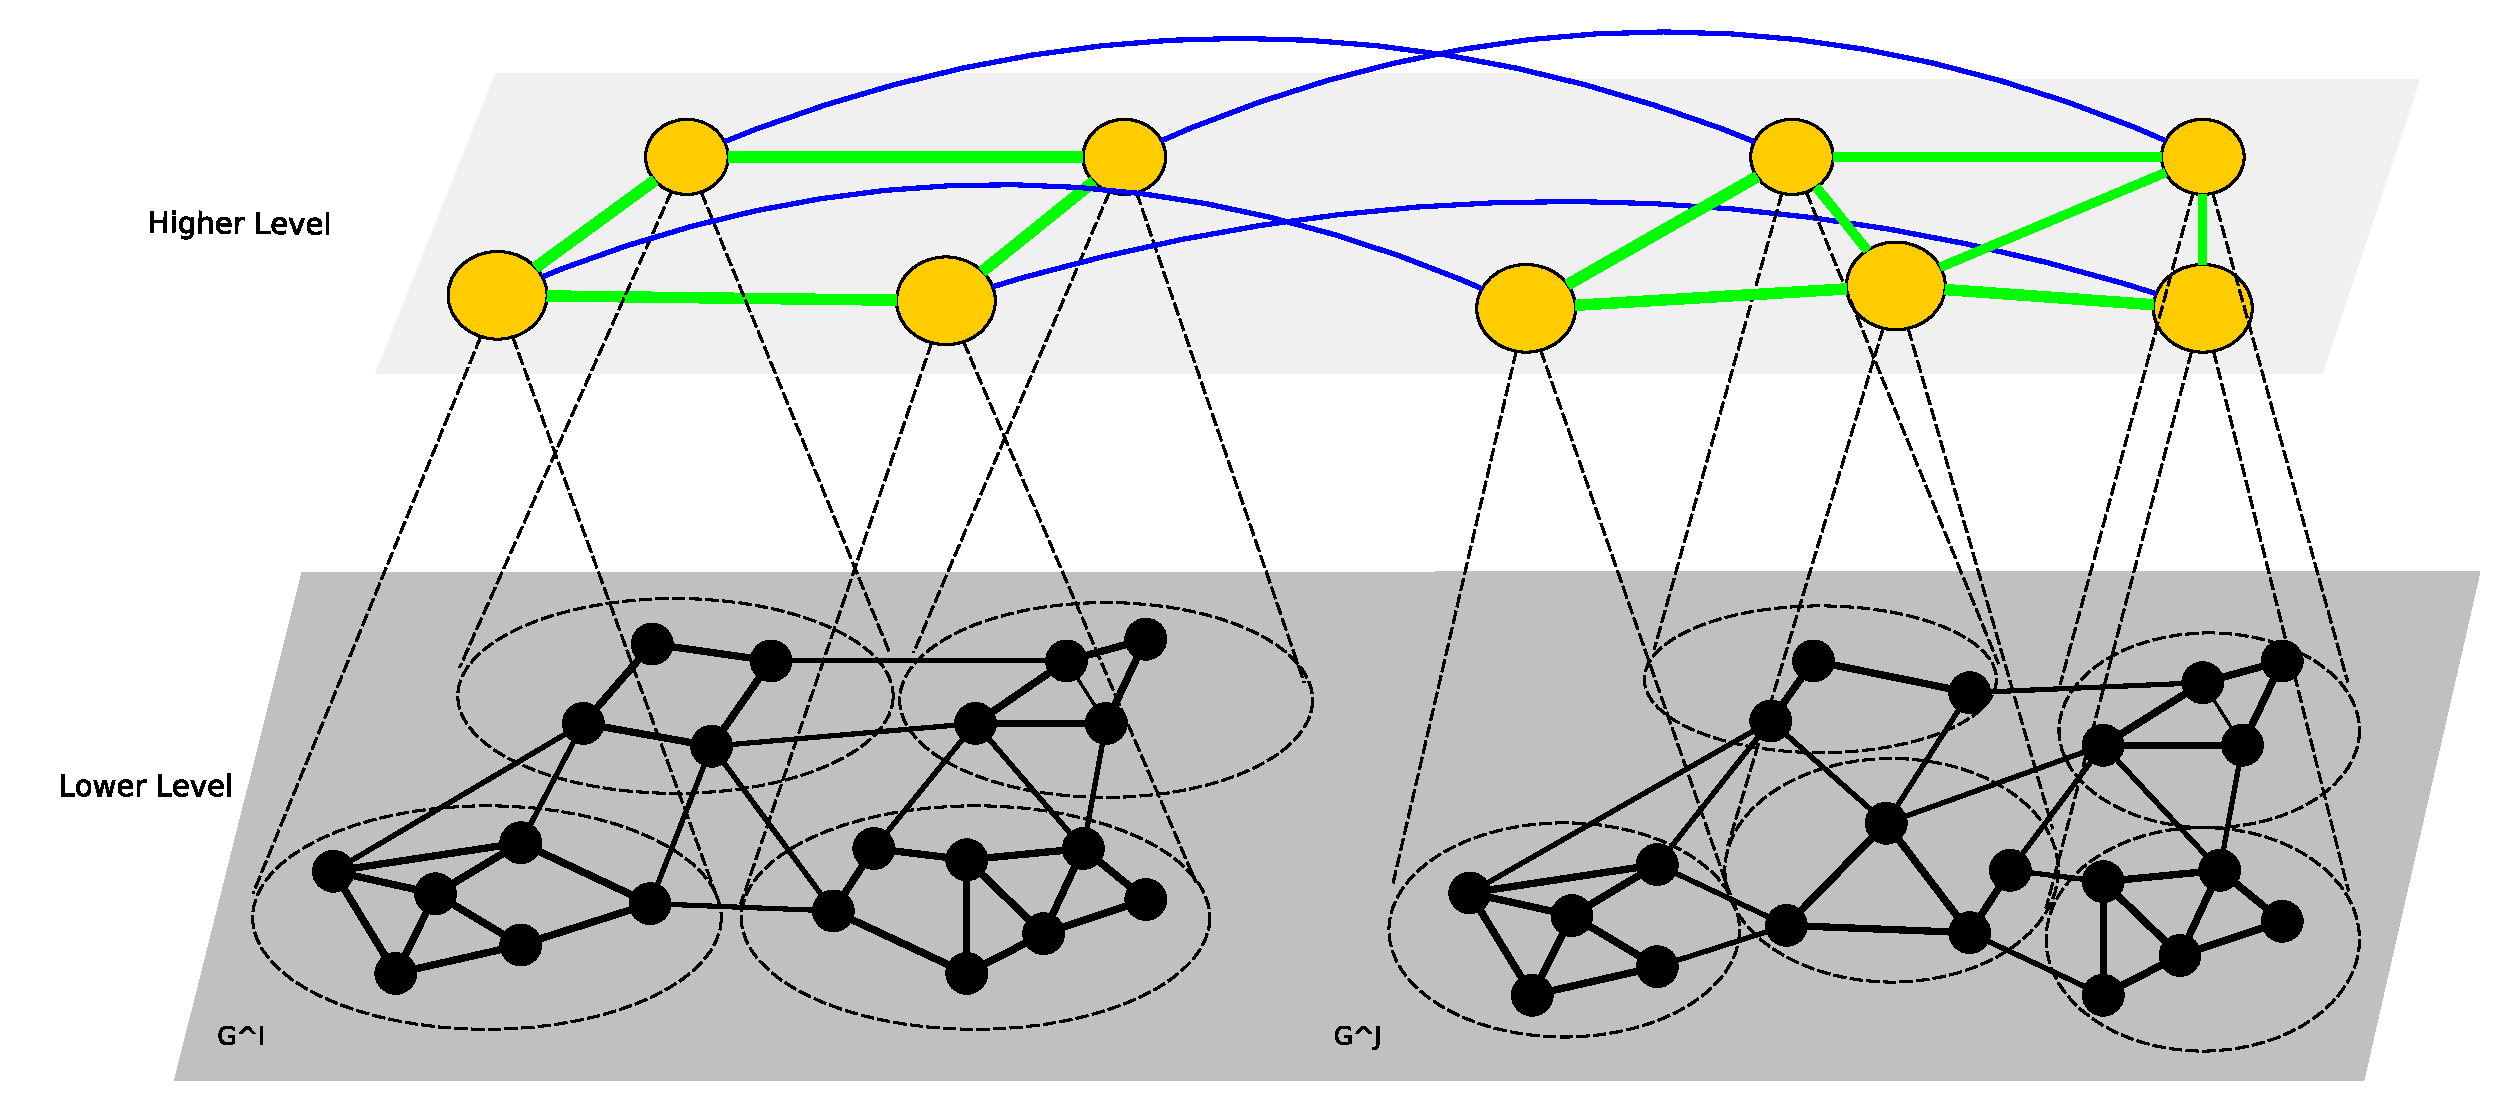
\includegraphics[scale=0.35]{fig/twolevels.pdf}
	\caption{Two level framework for graph matching} \label{fig:2levels}
\end{figure}

\FloatBarrier

% ------------------------------------------------------------------------------------------------------------
% ---------------------------------------        LLG Construction
\subsection{Lower Level Graph Construction}

In this section we describe the structure of lower level graphs built for given images $I$ and $J$.

Features, that were collected densely on the edges \cite{PMT}, represent the sets of nodes $V^I$, $V^J$ of the graphs $G^I$, $G^J$ respectively. This results in hundreds or thousand of nodes. As node attributes $D^I$, $D^J$ we used \emph{SIFT descriptors}~\cite{Lowe2004} with fixed orientation and scale. 

The nodes of the graphs are connected vie edges with their $k$ nearest neighbors.

To calculate the affinity matrix $S$ between two lower level graphs  $G^I$, $G^J$ or their subgraphs we need to define similarity functions between nodes and edges. Similarity of two nodes $v_i\in V^I, u_j\in V^J$ is equal to \emph{cosine similarity} of their descriptors.
For the pairwise edge similarity we used the same formula as in \cite{Cho2014_Haystack, Suh_CVPR2015}, i.e.\ 
\begin{equation}
s_E(e_{ii\prime}, e_{jj\prime}) = exp(-\frac{(l_{ii\prime} - l_{jj\prime})^2}{\sigma^2_{s}})
\label{eq:s_e}
\end{equation}
where $l_{ii\prime}$, $l_{jj\prime} $ are the lengths of edges $e_{ii\prime}\in E^I$ and $e_{jj\prime}\in E^J$ respectively.




% ------------------------------------------------------------------------------------------------------------
% ---------------------------------------        HLG Construction
\subsection{Higher Level Graph Construction}

%We define an anchor graph of a given fine graph $G = (V,E,D)$ as a $5-$tuple $A = (V^A,E^A,D_1^A,D_2^A,U^A)$, where $V^A$ is set of anchors, $E^{A}$ is set of edges between the anchors, $D_1^A$ and $D_2^A$ are two sets of anchor descriptors % based respectively on appearance  and structure of corresponding subgraphs
%and $U^{A}$ is correspondence matrix between anchors and nodes of $G$.

We define an anchor graph of a given fine graph $G = (V,E,D)$ as $A = (V^A,E^A, U^A)$, where $V^A$ is s set of anchors, $E^{A}$ is a set of edges between the anchors and $U^{A}$ is a correspondence matrix between anchors and nodes of $G$.

Each anchor $a_k\in V^A$ represent a subgraph $G_k = (V_k,E_k, D_k)$ of G. In case of $m$ anchors and $n$ nodes in $V$  matrix $U^{A}$ is a $n\times m$ binary matrix with 
$$U^{A}_{ik} = \begin{cases} 1, & \mbox{if node } v_i\in V_k    \\
	                         0, & \mbox{otherwise} \end{cases} $$	 
	                                                 
\subsubsection{Construction of anchor graph}	                         
To construct an anchor graph $A$ with fixed number $m$ of anchors from a given fine graph $G$ we adopted coarsening phase from multi-level graph partition algorithms \cite{Chevalier09_GP, Safro2012_GC, Karypis95_GP, Hendrickson1995}.
Such algorithms have three phases: 
\begin{enumerate}
	\item graph coarsening phase, where one creates a hierarchy of graphs by successive merging of nodes in graph on previous stage starting with initial graph;
	\item graph partition stage, where the partition problem is solved exact on the coarsest level;
	\item refinement phase, where solution of the coarsest level is interpolated through all levels of the hierarchy until the initial graph.
\end{enumerate}
There are several types of graph coarsening algorithms. In our work we used so-called strict aggregation scheme (\textbf{SAG}) \cite{Chevalier09_GP}, which groups nodes of $G$ in \emph{disjoint} subsets based on the strength of the edges between them. 

We implemented two SAG based algorithms: Heavy Edge Matching (\textbf{HEM}) and Light Edge Matching (\textbf{LEM})~\cite{Chevalier09_GP}. Both algorithms visit nodes of the $G$ in random order and construct a \emph{matching} $M$ of the graph. A selected node $v_i\in V(G)\setminus V(M)$ is matched to a node $v\prime\in V(G)\setminus V(M)$ in $M$, if $s_{vv\prime} = \max_{u\in N(v)} s_{vu}$ in case of HEM and
$s_{vv\prime} = \min_{u\in N(v)} s_{vu}$ in case of LEM. Here, $N(v)$ denotes the neighborhood of $v$, $V(M)$ the set of matched nodes and $s$ the strength of an edge. In case of LEM $s_{ii\prime} = l_{ii\prime}$ and in case of HEM $s_{ii\prime} = exp(-\frac{l_{ij}}{\sigma^2_{s}})$.

The edges in $M$ will be contracted, i.e.\ their endpoints will be replaced with a new node, that lies in the middle of a contracted edge and is connected to all neighbors of its endpoints.

It is clear, that one iteration of HEM or LEM reduces the number of nodes in $G$ at most by $\lfloor\frac{n}{2} \rfloor$ nodes. To get an coarse graph with $m$ nodes the coarsening algorithm should be repeated several times.

Obtained at the end coarse graph is the desired anchor graph $A$ of $G$. 

\subsubsection{Similarity matrix}

Assume, that for each of two given lower level graphs $G^I = (V^I, E^I, D^I)$ and $G^J=(V^J, E^J, D^J)$ we built the corresponding anchor graphs  $A^I=(V^{Ia},E^{Ia}, U^{Ia})$ and $A^J=(V^{Ja},E^{Ja},U^{Ja})$. 

We define the length of edges between two anchors $a_k$, $a_k\prime$ as a mean of distances between nodes in the corresponding subgraphs $G_k$ and $G_{k\prime}$. With other words:
\begin{equation} L_{kk\prime} = \median_{v_i\in G_k, v_{i\prime}\in G_{k\prime}} l_{ii\prime} \end{equation}
Based on this definition we use the same formula for \emph{edge similarity} between anchors as we set it for the lower level graphs (see Eq.\ref{eq:s_e}):
\begin{equation} 
s^A_E(e_{kk\prime}, e_{pp\prime}) = exp(-\frac{(L_{kk\prime} - L_{pp\prime})^2}{\sigma^2_{s}})
\label{eq:s_e_A}
\end{equation}
where $L_{kk\prime}$, $L_{pp\prime} $ are the lengths of edges $e_{kk\prime}\in E^{Ia}$ and $e_{pp\prime}\in E^{Ja}$ respectively.

To measure \emph{similarity between the anchors} we  define two different descriptors of an anchor $a$.

The first descriptor $d_1(a)$ should measure the similarity of node descriptors in corresponding subgraphs. For this purpose we adopted \emph{Bag Of Feature Model} \ToDo{ref}: we built a common dictionary based on the descriptors in $D^I$ and $D^J$ and define $d_1(a)$ as a histogram of "codewords" in corresponding subgraphs.

The second descriptor $d_2(a)$ should describe the structure similarity of subgraphs. We define $d_2(a)$ as a set of histograms $\{d_2(a,v)\}$ of the nodes $v$ in the underlying subgraph of the anchor $a$. The histograms of nodes have the fix number of bins $b$ and represent a distribution of the length of the subgraph edges inside a small circle region around each node. 

The similarity value between two anchors can be calculated now based on the first or second type of anchor descriptors by calculation of a distance between histograms based on $\chi^2$ statistic test \cite{Weken2004_ChiSqTest}:
\begin{equation}
s^A_1(a_k, a_p) = \sum_{b_i\in B}\frac{(d_1(a_k)-d_1(a_p))^2}{(d_1(a_k)+d_1(a_p))}
\end{equation}

\begin{equation}
s^A_2(a_k, a_p) = \frac{1}{|V(G_k)|}\frac{1}{V(G_p)|}\sum_{v\in V(G_k)}\sum_{u\in V(G_p)} \big(\sum_{b_i\in B}\frac{(d_2(a_k,v)-d_2(a_p,u))^2}{(d_2(a_k,v)+d_2(a_p,u))}\big)
\end{equation}

In our framework we use a combination of both anchor similarity functions:
\begin{equation}
s^A(a_k, a_p) = s_1(a_k, a_p)+s_2(a_k, a_p) 
\end{equation}


% ------------------------------------------------------------------------------------------------------------
% ---------------------------------------        Matcing algorithm
\subsection{Matching Algorithm}

Generally, it is possible to use in our approach arbitrary graph matching algorithm for finding correspondences between anchors (higher level) and nodes (lower level). However we selected \emph{Reweighted Random Walks Method} (\textbf{RRWM})~\cite{Cho2010_RRWM}, as it shows high matching accuracy ($64.01\%$ in average) and is fast. Additionally, it	 suits well for finding common subgraph of two graphs in presence of outliers.

Important is, that the algorithm solves relaxed version of the initial problem (see section \ref{sec:prob_stat}), where constraints (\ref{QIP:3}),(\ref{QIP:4}) are dropped and the integrality constrain (\ref{QIP:2}) is replaced with $x\in \{0,1\}^{n_1n_2}$. We used \emph{greedy mapping} analog to \cite{Leordeanu2005}, instead of Hungarian algorithm used by the authors for discretization of continues solutions.

% ------------------------------------------------------------------------------------------------------------
% ---------------------------------------        Level connection
\subsection{Connection between two levels}
Assume, we solved the GMP on the higher level. That means, we know pairs of correspondences between the anchor nodes: $m^a = \{(a_k, a_p)\}, a_i\in V^{Ia}, a_p\in V^{Ja}$. Since each anchor represents a subgraph of the initial graph, $m^a$ defines at the same time the correspondences between the subgraphs of the initial graphs $G^I$ and $G^J$. Solution of the $GMP$ for each pair of the subgraphs gives us the desirable correspondences between the nodes of the original graphs ($m = \{(v_i, v_j)\}, v_i\in V^{I}, v_j\in V^{J}$).

As we already mentioned above, the quality of the resulting solution $m$ depends in our framework not only on the quality of the graph matching algorithm, but also on the graph partitioning algorithm. The Fig.~\ref{fig:badpartition} shows, that by the fixed partition the matching results will be very pure for all possible matches of the anchors.

\begin{figure}
	\centering
	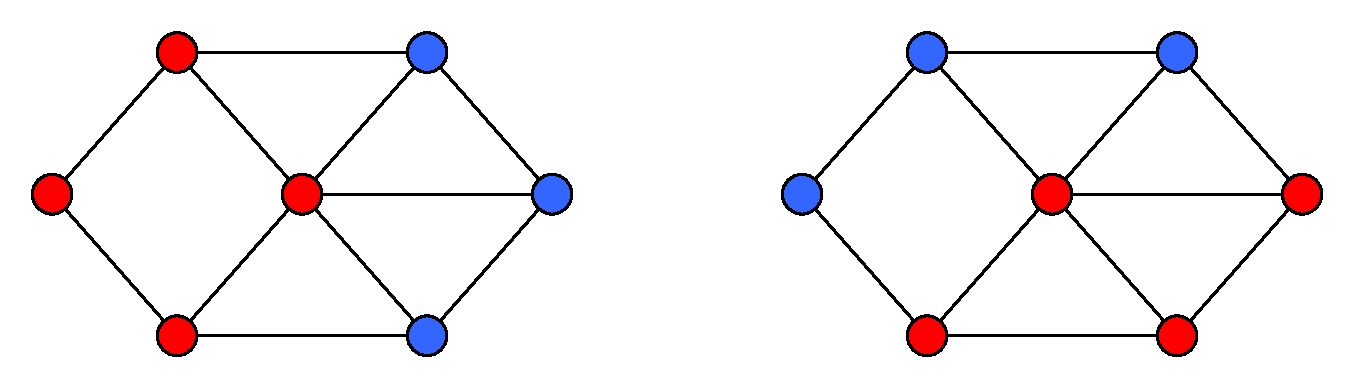
\includegraphics[scale=0.35]{fig/badpartition.pdf}
	\caption{Example of bad partition of two equal graphs into two subgraphs} \label{fig:badpartition}
\end{figure}


To cope with this problem, we present an \emph{iterative approach}, where the subgraphs of the initial graphs are allowed to exchange nodes based on the solution $m$ after each iteration of two-level graph matching algorithm. Exchanging rules are based on the affine transformations assigned to each matched pair of the subgraphs.

We consider two matched subgraphs $G^I_k=(V^I_k, E^I_k, D^I_k)$ and  $G^J_p=(V^J_p, E^J_p, D^J_p)$. Based on the matching between the nodes of this pair we apply \emph{RANSAC}~\cite{RANSAC} to estimate two \emph{affine transformations} $T_{kp}:V^I_k\rightarrow V^J_p$ and $T_{pk}:V^J_p\rightarrow V^I_k$. From this two transformations we select the one with smaller transformation error. The transformation error is defined as follows. For each node $v_i\in V^I_k$ we calculate the error between its matched node $m(v_i) = v_j\in V^J_p$ and its projection $T_{kp}(v_i)$: 
\begin{equation} \label{eq:err_v}
err(v_i) = \|T_kp(v_i) - m(v_i)\|_{l_2}
\end{equation}
The error of the estimated affine transformation $T_{kp}$ (analog for  $err(T_{pk})$) is then defined as
\begin{equation} \label{eq:err_T}
err(T_{kp}) = \median_{v_i\in V^I_k}err(v_i)
\end{equation}

For the transformation with the smallest error we calculate its inverse transformation and associate both of them with the subgraph match $(a_k, a_p)$. For simplicity we preserve the notation $T_{kp}$ and $T_{pk}$ for the transformations related to the subgraph match $(a_k, a_p)$.

In this way we can associate to each subgraph pair with more than $3$ node correspondences \footnote{we need at least $3$ pair of correspondences to be able to estimate an affine transformation} the estimated affine transformation of their nodes.

\textit{Rule $1$}

If the transformation describes well the matching between the subgraphs nodes (i.e.\ the transformation error~\ref{eq:err_T} is small), then we include nodes near $T_{kp}(V^I)$, $T_{pk}(V^J)$ in corresponding subgraph with the confidence value equal to $e^{-\min(err(T_{kp}), err(T_{pk}))}$. If one node was selected by several subgraphs, it will be included in the subgraph with the biggest associated confidence value.

\textit{Rule $2$}

If there are subgraph with less then $3$ nodes, we shift this nodes to the subgraphs of their nearest neighbors. For this nodes $err(v)=M$ (see Eq.~\ref{eq:err_v}), where $M$ is some big constant. 

The described approach for subgraph reorganization is summarized in Algorithm~\ref{alg:update_subgraphs}.

\vspace{20pt}
\begin{algorithm}[H]
	\KwIn{ correspondence matrices between nodes of the initial\\
		   \hspace{45pt}graphs and anchors: $U^{Ia}$, $U^{Ja}$\\
		   \hspace{45pt}list of matches between the subgraphs: $m^a = \{(a_k, a_p)\}$;\\
   		   \hspace{45pt}list of estimated affine transformations for each matched \\
   		   \hspace{45pt}pair: $\{(T_{kp}, T_{pk})\}$ }
	\KwOut{new correspondence matrices $\hat{U}^{Ia}$, $\hat{U}^{Ja}$}
	\nl define subgraphs of the initial graphs based on the correspondence \\
	matrices $U^{Ia}$, $U^{Ja}$: $\{G^I_k\}$ and  $\{G^J_p\}$ \\
	\nl $\hat{U}^{Ia} = \frac{1}{2}U^{Ia}$, $\hat{U}^{Ja} = \frac{1}{2}U^{Ja}$ \\
	\nl \ForEach{matched subgraph pair $(a_k, a_p)$}
			{\eIf{$\left|V^I_k\right|\ge 3$ \textbf{AND} $\left|V^J_p\right|\ge 3$}
				{ 
			      $err = \min(err(T_{kp}), err(T_{pk}))$ \tcp*{ see equations \ref{eq:err_v}, \ref{eq:err_T}}
 			      \If{
 			      	 $\left| err\right| < \epsilon $}   %\tcp*{ matching is reliable}
			         {
%			          \tcc{ confidence of the included node to belong to considering subgraphs equals $\exp(-err)$ }
			          $\hat{U}^{Ja}(v, a_p) = \exp(-err)$ for $v\in T_{kp}(V^{I}_k)$ \\
   		 	          $\hat{U}^{Ia}(v, a_k) = \exp(-err)$ for $v\in T_{pk}(V^{J}_p)$ \\
   		 	         }
   		 	    }
    		 	{shift nodes of too small subgraphs into subgraphs, their nearest neighbors belong to} 
		    }			
	\nl  set in each row of  $\hat{U}^{Ia}$($\hat{U}^{Ja}$) the maximum element to $1$ and all other to $0$\\
	\Return $\hat{U}^{Ia}$, $\hat{U}^{Ja}$
	
	\caption{UpdateSubgraphs}    \label{alg:update_subgraphs}
\end{algorithm}

\FloatBarrier

\subsubsection{Simulated Annealing \textbf{SM}}

After some experiments we found out, that the iterative aproach based on the two-level graph matching and the Algorithm~\ref{alg:update_subgraphs} can stay trapped in local optima.
To cope with this we use additionally ideas of the \emph{Simulated Annealing}.

We consider each of the two graphs separately. In each iteration \emph{after application of the Algorithm~\ref{alg:update_subgraphs}} we randomly try to shift a node to one of its three nearest anchors. The energy state of the system is defined as $E = \sum_{v\in V}err(v)$ (see Eq.~\ref{eq:err_v}). After one node was shifted, the new energy state $E^{new}$ is calculated. Wenn $E^{new}<E$ the shifted node stays in its new subgraph. Otherwise, the move is accepted with the probability $exp(-\frac{E^{new}-E}{T})$, where $T = 1/{it}$ is the current temperature of the system and depends on the iteration number $it$. 

\emph{Afterwards} we apply again the Algorithm~\ref{alg:update_subgraphs}.

% ------------------------------------------------------------------------------------------------------------
% ---------------------------------------        Experimantal Evaluation
\section{Experimental Evaluation}

\begin{figure}[ht] 
	\begin{subfigure}[b]{0.5\textwidth}
		\centering
		\includegraphics[scale=0.35]{fig/method1/test1/LL_it6.jpg} 
		\caption{Without $SM$} 
	\end{subfigure}%% 
	\begin{subfigure}[b]{0.5\textwidth}
		\centering
		\includegraphics[scale=0.35]{fig/method2/test1/LL_it6.jpg} 
		\caption{With $SM$} 
	\end{subfigure} 
	\caption{Result of the two-level graph matching approach after $6$ iterations }
\end{figure}

\begin{figure}[ht] 
	\begin{subfigure}[b]{0.5\textwidth}
		\centering
		\includegraphics[scale=0.35]{fig/method1/test2/LL_it11.jpg} 
		\caption{Without $SM$} 
	\end{subfigure}%%
	\begin{subfigure}[b]{0.5\textwidth}
		\centering
		\includegraphics[scale=0.35]{fig/method2/test2/LL_it11.jpg} 
		\caption{With $SM$} 
	\end{subfigure} 
	\caption{Result of the two-level graph matching approach after $11$ iterations }	
\end{figure}

\begin{figure}[ht] 
	\begin{subfigure}[b]{0.5\textwidth}
		\centering
		\includegraphics[scale=0.35]{fig/method1/test3/LL_it13.jpg} 
		\caption{Without $SM$} 
	\end{subfigure}%% 
	\begin{subfigure}[b]{0.5\textwidth}
		\centering
		\includegraphics[scale=0.35]{fig/method2/test3/LL_it13.jpg} 
		\caption{With $SM$} 
	\end{subfigure} 
	\caption{Result of the two-level graph matching approach after $13$ iterations }
\end{figure}

\newpage
\begin{landscape}
	
\begin{table}
	[ht] \caption{Results of two-level Graph Matching Approach } \label{tab:stimuli}
	\begin{tabular}
		{|L{4cm}|L{3cm}|L{3cm}|L{6cm}|L{6cm}|} \hline
%		              & \multicolumn{2}{c|}Higher Level} & \multicolumn{2}{c|}{Lower Level} \\ 
		Initial Graps & Higher Level without SM  & Higher Leve with SM &  Lower Level without SM &  Lower Level with SM \\ \hline
		% first row
		\rule{0pt}{5cm}
		\parbox[t]{1em}{
			\includegraphics[scale = 0.2]{fig/initial_graphs1.jpg}}  & 
		\parbox[b]{1em}{
			\includegraphics[scale = 0.28]{fig/method1/test1/accuracy_HL.jpg}}  & 
		\parbox[b]{1em}{
			\includegraphics[scale = 0.28]{fig/method2/test1/accuracy_HL.jpg}}  &
		\parbox[b]{1em}{
			\includegraphics[scale = 0.28]{fig/method1/test1/accuracy_LL.jpg}}  &
		\parbox[b]{1em}{
			\includegraphics[scale = 0.28]{fig/method2/test1/accuracy_LL.jpg}} \\
		\hline	
		
		\hline

		% second row
		\rule{0pt}{5cm}
		\parbox[t]{1em}{
			\includegraphics[scale = 0.2]{fig/initial_graphs2.jpg}}  & 
		\parbox[b]{1em}{
			\includegraphics[scale = 0.28]{fig/method1/test2/accuracy_HL.jpg}}  & 
		\parbox[b]{1em}{
			\includegraphics[scale = 0.28]{fig/method2/test2/accuracy_HL.jpg}}  &
		\parbox[b]{1em}{
			\includegraphics[scale = 0.28]{fig/method1/test2/accuracy_LL.jpg}}  &
		\parbox[b]{1em}{
			\includegraphics[scale = 0.28]{fig/method2/test2/accuracy_LL.jpg}} \\
		\hline	

		% third row
		\rule{0pt}{5cm}
		\parbox[t]{1em}{
			\includegraphics[scale = 0.2]{fig/initial_graphs3.jpg}}  & 
		\parbox[b]{1em}{
			\includegraphics[scale = 0.28]{fig/method1/test3/accuracy_HL.jpg}}  & 
		\parbox[b]{1em}{
			\includegraphics[scale = 0.28]{fig/method2/test3/accuracy_HL.jpg}}  &
		\parbox[b]{1em}{
			\includegraphics[scale = 0.28]{fig/method1/test3/accuracy_LL.jpg}}  &
		\parbox[b]{1em}{
			\includegraphics[scale = 0.28]{fig/method2/test3/accuracy_LL.jpg}} \\
		\hline			
		
	\end{tabular}
\end{table}


\end{landscape}

% ------------------------------------------------------------------------------------------------------------
% ---------------------------------------        Bibliography
\bibliographystyle{abbrv}
\bibliography{bibliography}
	
\end{document}